% Options for packages loaded elsewhere
\PassOptionsToPackage{unicode}{hyperref}
\PassOptionsToPackage{hyphens}{url}
%
\documentclass[
]{article}
\usepackage{lmodern}
\usepackage{amssymb,amsmath}
\usepackage{ifxetex,ifluatex}
\ifnum 0\ifxetex 1\fi\ifluatex 1\fi=0 % if pdftex
  \usepackage[T1]{fontenc}
  \usepackage[utf8]{inputenc}
  \usepackage{textcomp} % provide euro and other symbols
\else % if luatex or xetex
  \usepackage{unicode-math}
  \defaultfontfeatures{Scale=MatchLowercase}
  \defaultfontfeatures[\rmfamily]{Ligatures=TeX,Scale=1}
\fi
% Use upquote if available, for straight quotes in verbatim environments
\IfFileExists{upquote.sty}{\usepackage{upquote}}{}
\IfFileExists{microtype.sty}{% use microtype if available
  \usepackage[]{microtype}
  \UseMicrotypeSet[protrusion]{basicmath} % disable protrusion for tt fonts
}{}
\makeatletter
\@ifundefined{KOMAClassName}{% if non-KOMA class
  \IfFileExists{parskip.sty}{%
    \usepackage{parskip}
  }{% else
    \setlength{\parindent}{0pt}
    \setlength{\parskip}{6pt plus 2pt minus 1pt}}
}{% if KOMA class
  \KOMAoptions{parskip=half}}
\makeatother
\usepackage{xcolor}
\IfFileExists{xurl.sty}{\usepackage{xurl}}{} % add URL line breaks if available
\IfFileExists{bookmark.sty}{\usepackage{bookmark}}{\usepackage{hyperref}}
\hypersetup{
  pdftitle={Using long-term survey data to predict blue crab (Callinectes sapidus) abundance and commercial landings in Charleston Harbor, South Carolina},
  pdfauthor={Stephen R. Czwartacki; Michael R. Kendrick},
  hidelinks,
  pdfcreator={LaTeX via pandoc}}
\urlstyle{same} % disable monospaced font for URLs
\usepackage[margin=1in]{geometry}
\usepackage{graphicx,grffile}
\makeatletter
\def\maxwidth{\ifdim\Gin@nat@width>\linewidth\linewidth\else\Gin@nat@width\fi}
\def\maxheight{\ifdim\Gin@nat@height>\textheight\textheight\else\Gin@nat@height\fi}
\makeatother
% Scale images if necessary, so that they will not overflow the page
% margins by default, and it is still possible to overwrite the defaults
% using explicit options in \includegraphics[width, height, ...]{}
\setkeys{Gin}{width=\maxwidth,height=\maxheight,keepaspectratio}
% Set default figure placement to htbp
\makeatletter
\def\fps@figure{htbp}
\makeatother
\setlength{\emergencystretch}{3em} % prevent overfull lines
\providecommand{\tightlist}{%
  \setlength{\itemsep}{0pt}\setlength{\parskip}{0pt}}
\setcounter{secnumdepth}{-\maxdimen} % remove section numbering
\usepackage{booktabs}
\usepackage{longtable}
\usepackage{array}
\usepackage{multirow}
\usepackage{wrapfig}
\usepackage{float}
\usepackage{colortbl}
\usepackage{pdflscape}
\usepackage{tabu}
\usepackage{threeparttable}
\usepackage{threeparttablex}
\usepackage[normalem]{ulem}
\usepackage{makecell}
\usepackage{xcolor}

\title{Using long-term survey data to predict blue crab (\emph{Callinectes
sapidus}) abundance and commercial landings in Charleston Harbor, South
Carolina}
\usepackage{etoolbox}
\makeatletter
\providecommand{\subtitle}[1]{% add subtitle to \maketitle
  \apptocmd{\@title}{\par {\large #1 \par}}{}{}
}
\makeatother
\subtitle{14Mar2020 edit: 2}
\author{Stephen R. Czwartacki \and Michael R. Kendrick}
\date{}

\begin{document}
\maketitle
\begin{abstract}
Marked high fluctuations in blue crab (\emph{Callinectes sapidus})
seasonal and annual abundance, and commercial landings are typical, but
data from both fisheries independent and dependent surveys have shown
declines in populations in recent years in South Carolina. Despite
several long-term fisheries independent surveys encountering blue crab,
predictive models have not recently been developed in South Carolina to
quantify variation in abundance and commercial landings. The goal of
this study is to assess the current status of blue crab in SC and
explore the potential for developing a more predictive understanding of
commercial landings. This goal is met through the following objectives:
1) assess long-term trends in blue crab landings and
fisheries-independent abundance, 2) test the applicability of a juvenile
index, where juvenile abundance in one year predicts adult abundance in
a subsequent years (e.g.~1-yr and 2-yr lag), 3) explore other indices of
abundance for size class and sexual maturity categories as they relate
to total or adult blue crab abundance in subsequent years (e.g.~1-yr and
2-yr lag), and 4) explore predictive relationships between
fisheries-independent size class and sexual maturity abundance
categories and commercial landings. Data from several long-term South
Carolina Department of Natural Resources (SCDNR) fisheries independent
blue crab surveys were standardized for each of six surveys and
commercial landings data were compiled. Analyses testing the application
of a juvenile index of abundance show that no juveniles collected in
surveys explain variation in annual survey abundances. The Creek Trawl
survey was the only survey with significant, but weak, correlative
relationships between multiple lagged population structure variables and
its own annual adult or total abundance. Significant relationships were
found with effort-corrected commercial landings predicted by the
previous year's abundance of male crabs. This relationship was most
correlated for immature crabs collected in the Harbor Trawl survey, and
for mature crabs collected in the Creek Trawl survey. These results
suggest a larger influence on abundance of blue crab from fishing effort
than population dynamics, and a potential influence from other external
factors such as habitat or environmental variables.
\end{abstract}

{
\setcounter{tocdepth}{2}
\tableofcontents
}
\newpage

\hypertarget{background}{%
\subsection{Background}\label{background}}

The blue crab (Callinectes sapidus) is a highly ranked commercial and
recreational fishery in South Carolina with 3.9 million lbs landed and a
value of \$5.1 million in 2018. To support management, it is important
to understand recruitment dynamics of juvenile blue crab into the adult
stage -- the stage that is available to commercial and recreational
fishers. Models can be developed to assess recruitment dynamics,
including testing of crab abundance in any given year and its
relationship to crab abundance in preceding years. If adult abundance in
a year is predicted by juvenile abundance in the prior year (e.g., 1-yr
lag), this may provide a more predictive understanding of the blue crab
fishery. The South Carolina Department of Natural Resources (SCDNR)
monitors the status of juvenile and adult blue crab across a range of
habitat types using multiple fisheriesindependent surveys.

\newpage

\hypertarget{methods}{%
\subsection{Methods}\label{methods}}

\hypertarget{survey-methods}{%
\subsubsection{Survey Methods}\label{survey-methods}}

A suite of fisheries independent monitoring surveys employed by the
South Carolina Department of Natural Resources (SCDNR) encounter the
blue crab using varying gear types in varying habitats with varying
sampling regimes (Table 1).

Biotic data recorded as part of both surveys (size, sex, maturity). Size
is determined by measurement of the carapace width. Sex and maturity are
determined by presence of morphological characteristics of the abdomen.

\hypertarget{analytical-mehods}{%
\subsubsection{Analytical Mehods}\label{analytical-mehods}}

Data were put through a rigorous data wrangling process to standardize
each survey relative to its own methods. Fisheries dependent commercial
landings and fisheries independent survey abundances were truncated from
statewide data to Charleston Harbor watershed data. Individual crabs
were assigned to the following size and sexual maturity categories
(Table 2): Size Classes - juvenile (\textgreater59mm), subadult (61mm -
126mm), sublegal (\textless127mm) and adult (\textgreater126mm); Sexual
maturity classes: mature female, immature female, mature male, and
immature male. Monthly means across all stations were used to calculate
mean annual abundances as catch-per-unit-effort (CPUE). Adult CPUEs were
compared to juvenile CPUEs 1 and 2 years prior to test the applicability
of a juvenile index. Additional indices of adult CPUE and total CPUE
were developed using single regression models (n=) for each life-stage
specific category at 1-yr and 2-yr lags. Significant (\(\alpha\) = 0.05)
models were ranked by explanatory power (i.e., r\textsuperscript{2})

\newpage

\textbf{Table 1:} SCDNR fisheries independent survey methodology.\\

\begin{table}[H]
\centering\begingroup\fontsize{8}{10}\selectfont

\resizebox{\linewidth}{!}{
\begin{tabular}{ll>{\raggedright\arraybackslash}p{6em}>{\raggedright\arraybackslash}p{6em}>{\raggedright\arraybackslash}p{6em}>{\raggedright\arraybackslash}p{6em}>{\raggedleft\arraybackslash}p{5em}>{\raggedright\arraybackslash}p{7em}}
\toprule
\multicolumn{1}{c}{ } & \multicolumn{2}{c}{Gear} & \multicolumn{3}{c}{Sample} & \multicolumn{2}{c}{Data} \\
\cmidrule(l{3pt}r{3pt}){2-3} \cmidrule(l{3pt}r{3pt}){4-6} \cmidrule(l{3pt}r{3pt}){7-8}
Survey & Gear Method & Gear Type & Sample Area & Sample Interval & Sample Method & N(events) & CPUE Standardization\\
\midrule
\addlinespace[0.3em]
\multicolumn{8}{l}{\textbf{CRMS}}\\
\hspace{1em}Creek Trawl & Active & 6m Trawl, 2.54cm stretch mesh & Ashley River, Wando River & Monthly, May-Sep & Fixed Stations & 1827 & Time\\
\hspace{1em}Harbor Trawl & Active & 4.6m Trawl, 0.6cm D mesh & Ashley River, Charleston Harbor & Monthly & Fixed Stations & 2956 & Time, Gear\\
\hspace{1em}Ashley Fall Potting & Passive & 0.6 x 0.6 x 0.46m Pot, 3.8 cm mesh & Ashley River & Monthly, Oct-Nov & Randomized Block w/in a Fixed Station & 128 & Time\\
\addlinespace[0.3em]
\multicolumn{8}{l}{\textbf{ERS}}\\
\hspace{1em}SCECAP Tidal Creeks & Active & 5m trawl, 1.9cm bar mesh & Charleston Harbor Systemwide & Jun - Aug & Random Stratified & 62 & Volumetric\\
\hspace{1em}SCECAP Open Water & Active & 5m trawl, 1.9cm bar mesh & Charleston Harbor Systemwide & Jun - Aug & Random Stratified & 92 & Volumetric\\
\addlinespace[0.3em]
\multicolumn{8}{l}{\textbf{IFRS}}\\
\hspace{1em}Trammel Net & Passive & 183 x 2.1m trammel net & Charleston Harbor Systemwide & Monthly & Random Stratified & 4736 & None (Total)\\
\bottomrule
\end{tabular}}
\endgroup{}
\end{table}

\textbf{Table 2:} Blue crab size class and sexual maturity data found in
SCDNR fisheries independent surveys\\

\begin{table}[H]
\centering\begingroup\fontsize{8}{10}\selectfont

\resizebox{\linewidth}{!}{
\begin{tabular}{lccccccccc}
\toprule
\multicolumn{2}{c}{ } & \multicolumn{4}{c}{Size} & \multicolumn{4}{c}{Class (Sex/Maturity)} \\
\cmidrule(l{3pt}r{3pt}){3-6} \cmidrule(l{3pt}r{3pt}){7-10}
Survey & Total CPUE & Juvenile & Subadult & Sublegal & Adult & Immature Female & Mature Female & Immature Male & Mature Male\\
\midrule
\addlinespace[0.3em]
\multicolumn{10}{l}{\textbf{CRMS}}\\
\hspace{1em}Creek Trawl & X & X & X & X & X & X & X & X & X\\
\hspace{1em}Harbor Trawl & X & X & X & X & X & X & X & X & X\\
\hspace{1em}Ashley Fall Potting & X &  &  & X & X &  &  &  & \\
\addlinespace[0.3em]
\multicolumn{10}{l}{\textbf{ERS}}\\
\hspace{1em}SCECAP Tidal Creeks & X & X & X & X & X &  &  &  & \\
\hspace{1em}SCECAP Open Water & X & X & X & X & X &  &  &  & \\
\addlinespace[0.3em]
\multicolumn{10}{l}{\textbf{IFRS}}\\
\hspace{1em}Trammel Net & X &  &  &  &  &  &  &  & \\
\bottomrule
\end{tabular}}
\endgroup{}
\end{table}

\newpage

\hypertarget{restults}{%
\section{Restults}\label{restults}}

\hypertarget{objective-1}{%
\subsection{Objective 1}\label{objective-1}}

\emph{Assess long-term trends in blue crab landings and
fisheries-independent abundance}

Time series of mean annual commercial landings (Fig. 1) and adult
abundances from SCDNR fisheries independent surveys (fig.~2) show the
high inter-annual variablility of legal-sized ``adult'' blue crab
(\textgreater126mm). These figures both show crab \textgreater126mm,
which is the minimum legal limit of blue crab in South Carolina.

The total pounds landed in the combined Charleston Harbor watersheds
shows a trending decline from 2003 - 2010, but when these same landings
data are corrected for effort in terms of number of pots pulled that
trend is not observed. The year 2003 marks the first year of ``trip
ticket'' reporting, in which all commercial blue crab license holders
are required to report their catch. This is the same time
(\textgreater2003) landings data have incorporated data from the Ashley
River and Cooper River reporting areas. This could be due to not being
actively fished for blue crab, underreported for these reporting areas
or included in another reporting area (e.g.~a line of crab pots
beginning in the Ashley River and continuing into Charleston Harbor
where landings are eventually reported). Adult abundances from some
surveys (B-Creek Trawl, C-Ashley Potting and D-SCECAP Open-Water) show a
slight decline in adult abundance shortly after 2000.

\begin{figure}
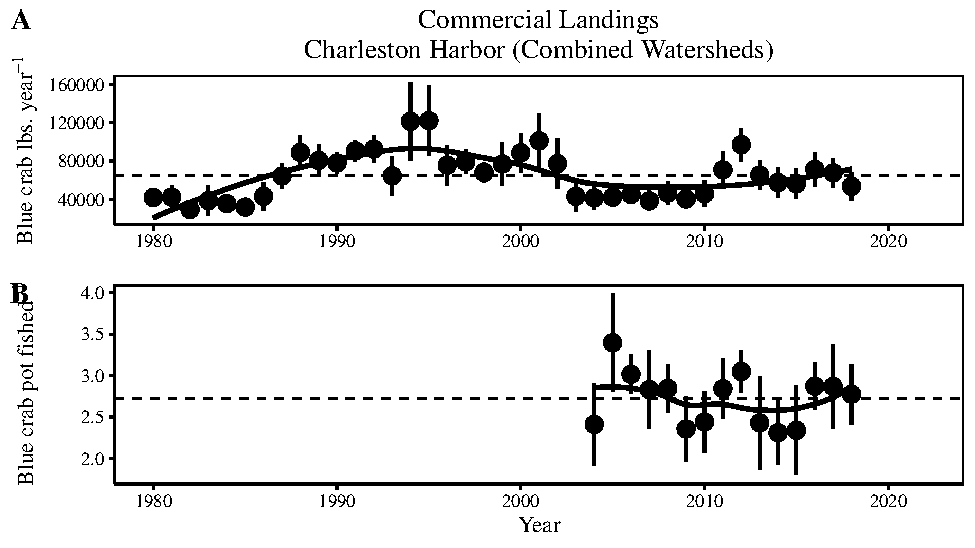
\includegraphics[width=0.75\linewidth]{NEWCh1_Figs_files/figure-latex/Figure 1-1} \caption{Plot represents mean annual time series of (A) total landings in total lbs./yr and (B) mean annual effort-corrected landings (total lbs./pot pulled/yr) for the combined reporting areas of the Charleston Harbor watershed}\label{fig:Figure 1}
\end{figure}

\begin{figure}
\centering
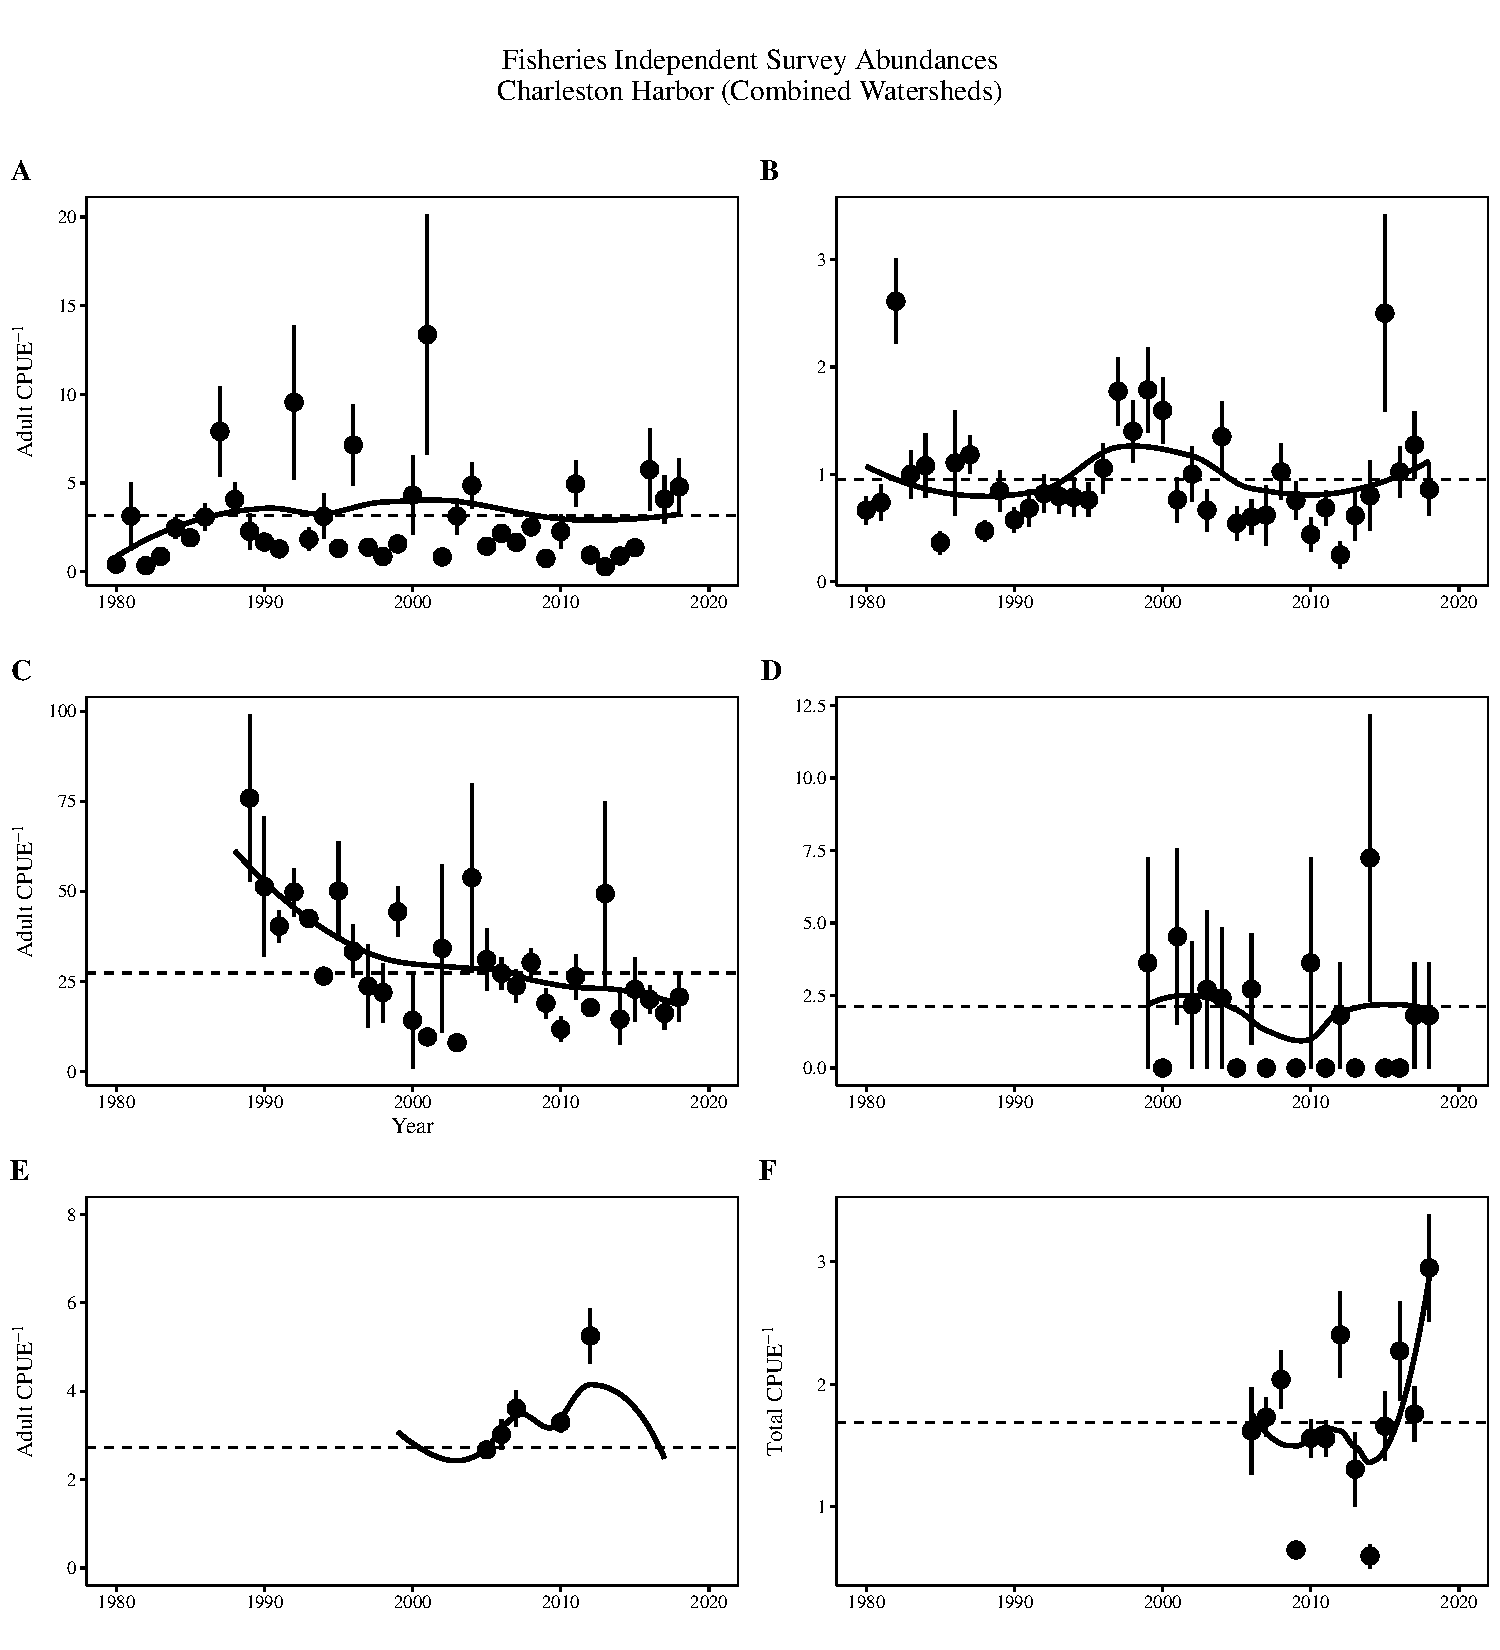
\includegraphics{NEWCh1_Figs_files/figure-latex/Figure 2 (CRMS Survey Time Series)-1.pdf}
\caption{Plot represents mean annual adult survey abundances of the (A)
Harbor Trawl, (B) Creek Trawl, (C) Ashley Potting Survey, (D) SCECAP
Open-Water and (E) SCECAP Tidal-Creek surveys, with standard error,
long-term mean (dashed) and a LOESS smoothing line (solid). The Tammel
Net survey does not have size or sexual maturity data and is represented
by total CPUE in this plot.}
\end{figure}

\newpage

\hypertarget{objective-2}{%
\subsection{Objective 2}\label{objective-2}}

\emph{Test the applicability of a juvenile index, where juvenile
abundance in one year predicts adult abundance in a subsequent years
(e.g.~1-yr and 2-yr lag)}

Mean annual juvenile CPUE is not significantly related to mean annual
adult CPUE in subsequent years for any survey (Table 3).

\textbf{Table 3:} Insignificant and poorly correlated relationships of
adult CPUEs by juvenile CPUEs

\begin{table}[H]
\centering\begingroup\fontsize{10}{12}\selectfont

\begin{tabular}{ll>{\centering\arraybackslash}p{4em}>{\centering\arraybackslash}p{4em}>{\centering\arraybackslash}p{6em}}
\toprule
\multicolumn{2}{c}{ } & \multicolumn{3}{c}{Summary Statistics} \\
\cmidrule(l{3pt}r{3pt}){3-5}
Dpendent Variable & Explanatory Variable & p-value & r2 & Degrees of Freedom\\
\midrule
\addlinespace[0.3em]
\multicolumn{5}{l}{\textbf{Harbor Trawl}}\\
\hspace{1em}Adult & Juvenile (1-yr. lag) & 0.15 & 0.06 & 36\\
\hspace{1em}Adult & Juvenile (2-yr. lag) & 0.86 & <0.01 & 35\\
\addlinespace[0.3em]
\multicolumn{5}{l}{\textbf{Creek Trawl}}\\
\hspace{1em}Adult & Juvenile (1-yr. lag) & 0.43 & 0.02 & 36\\
\hspace{1em}Adult & Juvenile (2-yr. lag) & 0.35 & 0.02 & 35\\
\addlinespace[0.3em]
\multicolumn{5}{l}{\textbf{SCECAP Open Water}}\\
\hspace{1em}Adult & Juvenile (1-yr. lag) & 0.19 & 0.11 & 36\\
\hspace{1em}Adult & Juvenile (2-yr. lag) & 0.15 & 0.14 & 35\\
\addlinespace[0.3em]
\multicolumn{5}{l}{\textbf{SCECAP Tidal Creek}}\\
\hspace{1em}Adult & Juvenile (1-yr. lag) & 0.77 & <0.01 & 36\\
\hspace{1em}Adult & Juvenile (2-yr. lag) & 0.24 & 0.14 & 35\\
\addlinespace[0.3em]
\multicolumn{5}{l}{\textbf{Ashley Potting}}\\
\hspace{1em}Legal (adult) & Sublegal (1-yr. lag) & 0.34 & 0.03 & 36\\
\hspace{1em}Legal (adult) & Sublegal (2-yr. lag) & 0.56 & 0.01 & 35\\
\bottomrule
\end{tabular}
\endgroup{}
\end{table}

\newpage

\hypertarget{objective-3}{%
\subsection{Objective 3}\label{objective-3}}

\emph{Explore other indices of abundance for size class and sexual
maturity categories as they relate to total or adult blue crab abundance
in subsequent years (e.g.~1-yr and 2-yr lag)}

The CRMS Creek Trawl is the only survey (see notes for Tables 5 \& 6)
with predictive relationships where size class and sexual maturity
categories relate to total or adult abundance in succesive years (Table
4). Fifteen size class and sexual maturity variables with 1- and 2-yr
lag explain total CPUE and explain adult CPUE. The highest ranked model
total Creek Trawl CPUE explained by subadult CPUE with a 2-yr lag
(\emph{p}-value = \textless0.01, r\textsuperscript{2} = 0.24; Fig. 3).

\textbf{Table 4:} These are all relevant explanatory variables
predicting CRMS Creek Trawl Survey total and adult CPUEs

\begin{table}[H]
\centering\begingroup\fontsize{10}{12}\selectfont

\begin{tabular}{ll>{\centering\arraybackslash}p{6em}>{\centering\arraybackslash}p{6em}>{\centering\arraybackslash}p{6em}}
\toprule
\multicolumn{2}{c}{ } & \multicolumn{3}{c}{Summary Statistics} \\
\cmidrule(l{3pt}r{3pt}){3-5}
Dependent Variable & Explanatory Variable & p-value & r2 & Degrees of Freedom\\
\midrule
Total CPUE & Subadult (2-yr. lag) & <0.01 & 0.24 & 35\\
Total CPUE & Mature Male (1-yr. lag) & <0.01 & 0.23 & 36\\
Total CPUE & Immature Male (2-yr. lag) & <0.01 & 0.21 & 35\\
Total CPUE & Sublegal (1-yr. lag) & <0.01 & 0.21 & 35\\
Total CPUE & Total CPUE (2-yr lag) & <0.01 & 0.21 & 35\\
\addlinespace
Total CPUE & Subadult (1-yr. lag) & <0.01 & 0.18 & 36\\
Total CPUE & Immature Female (2-yr. lag) & <0.01 & 0.17 & 35\\
Total CPUE & Mature Female (2-yr lag) & <0.05 & 0.15 & 35\\
Total CPUE & Total CPUE (1-yr lag) & <0.05 & 0.14 & 36\\
Total CPUE & Sublegal (1-yr. lag) & <0.05 & 0.13 & 36\\
\addlinespace
Total CPUE & Mature Male (2-yr. lag) & <0.05 & 0.13 & 35\\
Total CPUE & Adult (1-yr. lag) & <0.05 & 0.12 & 36\\
Total CPUE & Legal (1-yr. lag) & <0.05 & 0.12 & 36\\
Total CPUE & Immature Male (1-yr. lag) & <0.05 & 0.10 & 36\\
Total CPUE & Immature Female (1-yr. lag) & <0.05 & 0.10 & 36\\
\hline
\addlinespace
Adult CPUE & Mature Male (1-yr. lag) & <0.01 & 0.16 & 36\\
Adult CPUE & Mature Female (2-yr lag) & <0.05 & 0.12 & 35\\
\bottomrule
\end{tabular}
\endgroup{}
\end{table}

\begin{figure}
\centering
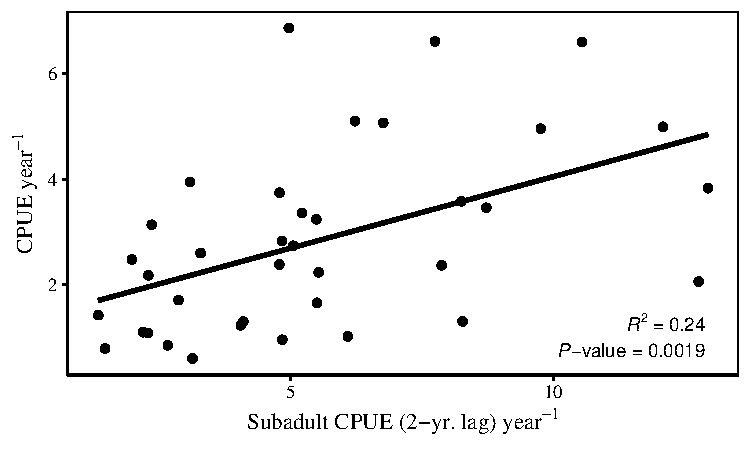
\includegraphics{NEWCh1_Figs_files/figure-latex/Figure 3 (Sub Plot)-1.pdf}
\caption{Plot showing the regression relationship of total Creek Trawl
CPUE by Creek Trawl subadult CPUE from 2 years prior. This the highest
correlated relationship of total or adult CPUE by lagged lifestage
variable.}
\end{figure}

\newpage

\hypertarget{tables-5-6}{%
\subsubsection{Tables 5 \& 6}\label{tables-5-6}}

The SCECAP Tidal Creek survey has multiple very significant and highly
correlative relationships with size and sexual maturity categories
predicting total and adult CPUEs, but I would like it removed from the
analyses. Constructing regression models using the same methodology as
the other surveys makes SCECAP Tidal Creeks trawl look like a super star
at first glance, with ridiculously high r\textsuperscript{2}'s (Table
5). But there are a max of 6 sampling events/year (mean sampling events
= 3.1) and never greater than 4 events after 2005 (Table 6). SCECAP
Tidal Creek survey only has a total of 192 crab caught (135 in 2012)
over the life of the survey with an inflated CPUEs based-on volumetric
standardization of SCECAP's catch.

\textbf{Tables 5}: OLS regression results of SCECAP total and adult CPUE
by all lifestages from SCECAP Tidal Creek survey

\begin{table}[H]
\centering\begingroup\fontsize{10}{12}\selectfont

\begin{tabular}{ll>{\centering\arraybackslash}p{6em}>{\centering\arraybackslash}p{6em}>{\centering\arraybackslash}p{6em}}
\toprule
\multicolumn{2}{c}{ } & \multicolumn{3}{c}{Summary Statistics} \\
\cmidrule(l{3pt}r{3pt}){3-5}
Dependent Variable & Explanatory Variable & p-value & r2 & Degrees of Freedom\\
\midrule
\addlinespace[0.3em]
\multicolumn{5}{l}{\textbf{SCECAP Tidal Creek}}\\
\hspace{1em}Total CPUE & Subadult (2-yr. lag) & <0.001 & 0.93 & 10\\
\hspace{1em}Total CPUE & Sublegal (2-yr. lag) & <0.001 & 0.92 & 10\\
\hspace{1em}Total CPUE & Total CPUE (2-yr lag) & <0.001 & 0.88 & 10\\
\hspace{1em}Total CPUE & Adult (2-yr. lag) & <0.01 & 0.54 & 10\\
\hline
\hspace{1em}Adult CPUE & Subadult (2-yr. lag) & <0.001 & 0.91 & 10\\
\hspace{1em}Adult CPUE & Sublegal (2-yr. lag) & <0.001 & 0.90 & 10\\
\hspace{1em}Adult CPUE & Total CPUE (2-yr lag) & <0.001 & 0.85 & 10\\
\hspace{1em}Adult CPUE & Adult (2-yr. lag) & <0.01 & 0.51 & 10\\
\addlinespace[0.3em]
\multicolumn{5}{l}{\textbf{SCECAP Open Water}}\\
\hspace{1em}Adult CPUE & Adult (1-yr lag) & <0.05 & 0.24 & 10\\
\bottomrule
\end{tabular}
\endgroup{}
\end{table}

\newpage

\textbf{Tables 6}: SCECAP Tidal Creek survey data table showing a small
annual sample size with small raw abundance numbers, inflated CPUEs and
several years with no sampling events

\begin{table}[H]
\centering\begingroup\fontsize{10}{12}\selectfont

\begin{tabular}{l>{\raggedright\arraybackslash}p{6em}>{\centering\arraybackslash}p{6em}>{\centering\arraybackslash}p{4em}>{\centering\arraybackslash}p{4em}>{\centering\arraybackslash}p{4em}>{\raggedright\arraybackslash}p{4em}}
\toprule
Year & Sampling Events & Raw Abundance & Total CPUE & Juvenile CPUE & Subadult CPUE & Adult CPUE\\
\midrule
1999 & 6 & 4 & 9.7 & 0.0 & 7.2 & 2.4\\
2000 & 6 & 3 & 7.2 & 0.0 & 0.0 & 4.8\\
2001 & 4 & 1 & 3.6 & 0.0 & 0.0 & 3.6\\
2002 & 6 & 0 & 0.0 & 0.0 & 0.0 & 0.0\\
2003 & 6 & 2 & 4.8 & 0.0 & 4.8 & 0.0\\
\addlinespace
2004 & 4 & 2 & 7.2 & 0.0 & 3.6 & 3.6\\
2005 & 8 & 7 & 12.7 & 1.8 & 0.0 & 10.9\\
2006 & 2 & 3 & 21.7 & 0.0 & 0.0 & 21.7\\
2007 & 4 & 12 & 48.1 & 0.0 & 15.0 & 33.2\\
2008 & 2 & 0 & 0.0 & 0.0 & 0.0 & 0.0\\
\addlinespace
2009 & 0 &  &  &  &  & \\
2010 & 4 & 18 & 65.2 & 3.6 & 32.6 & 29.0\\
2011 & 0 &  &  &  &  & \\
2012 & 2 & 135 & 1291.1 & 0.0 & 1061.6 & 229.5\\
2013 & 0 &  &  &  &  & \\
\addlinespace
2014 & 0 &  &  &  &  & \\
2015 & 2 & 1 & 7.2 & 7.2 & 0.0 & 0.0\\
2016 & 2 & 1 & 7.2 & 0.0 & 0.0 & 7.2\\
2017 & 2 & 2 & 14.5 & 0.0 & 7.2 & 7.2\\
2018 & 2 & 1 & 7.2 & 0.0 & 7.2 & 0.0\\
\bottomrule
\end{tabular}
\endgroup{}
\end{table}

\newpage

\hypertarget{objective-4}{%
\subsection{Objective 4}\label{objective-4}}

\emph{Explore predictive relationships between fisheries-independent
size class and sexual maturity abundance categories and commercial
landings}

Nine total predictive models using several size class and sexual
maturity categories with 1-yr lag to explain effort corrected landings
were developed. No 2-yr lagged size class and sexual maturity categories
predict effort corrected landings. Predictive relationships were only
found using the CRMS Harbor Trawl (N = 3) and Creek Trawl (N = 6)
surveys. The strongest relationships ranked by explanatory power
(r\textsuperscript{2}) use the Harbor Trawl subadults with a 1-yr lag
(\emph{p} = \textless0.01, r\textsuperscript{2} = 0.43) and the Creek
Trawl immature males with a 1-yr lag (\emph{p} = \textless0.01,
r\textsuperscript{2} = 0.41; Table 7).

Total landings (not effort corrected) have only two predictive
relationships were size classs and sexual maturity variables from any
survey predict total annual lbs landed (Table 8). These two poorly
correlated relationships use mature males with a 1-yr lag from the
Harbor Trawl (\emph{p} = \textless0.05, r\textsuperscript{2} = 0.10) and
adults with a 2-yr lag from the Ashley Potting Survey (\emph{p} =
\textless0.05, r\textsuperscript{2} = 0.15) to predict total annual
pounds landed. Total landings data are missing for the Ashley and Cooper
Rivers prior to 2004.

\textbf{Table 7:} Objective 3 - All significant relatioships of effort
corrected Charleston Harbor watershed (Ashley, Cooper and Wando Rivers
and Charlesotn Harbor) commercial Landings by size classs and sexual
maturity variables from all surveys using OLS regression.

\begin{table}[H]
\centering\begingroup\fontsize{8}{10}\selectfont

\begin{tabular}{ll>{\centering\arraybackslash}p{4em}>{\centering\arraybackslash}p{4em}c}
\toprule
\multicolumn{2}{c}{ } & \multicolumn{3}{c}{Summary Statistics} \\
\cmidrule(l{3pt}r{3pt}){3-5}
Dependent Variable & Explanatory Variable & p-value & r2 & Degrees of Freedom\\
\midrule
\addlinespace[0.3em]
\multicolumn{5}{l}{\textbf{Harbor Trawl (explanatory variable)}}\\
\hspace{1em}Mean Landings (effort corrected) & Mature Male (1-yr. lag) & <0.01 & 0.43 & 13\\
\hspace{1em}Mean Landings (effort corrected) & Subadult (1-yr. lag) & <0.05 & 0.37 & 13\\
\hspace{1em}Mean Landings (effort corrected) & Total CPUE (1-yr. lag) & <0.05 & 0.32 & 13\\
\addlinespace[0.3em]
\multicolumn{5}{l}{\textbf{Creek Trawl (explanatory variable)}}\\
\hspace{1em}Mean Landings (effort corrected) & Immature Male (1-yr. lag) & <0.01 & 0.41 & 13\\
\hspace{1em}Mean Landings (effort corrected) & Sublegal (1-yr. lag) & <0.05 & 0.38 & 13\\
\hspace{1em}Mean Landings (effort corrected) & Subadult (1-yr. lag) & <0.05 & 0.35 & 13\\
\hspace{1em}Mean Landings (effort corrected) & Total CPUE (1-yr. lag) & <0.05 & 0.33 & 13\\
\hspace{1em}Mean Landings (effort corrected) & Juvenile (1-yr. lag) & <0.05 & 0.31 & 13\\
\hspace{1em}Mean Landings (effort corrected) & Immature Female (1-yr. lag) & <0.05 & 0.30 & 13\\
\bottomrule
\end{tabular}
\endgroup{}
\end{table}

\textbf{Table 8:} All significant relatioships of total Charleston
Harbor watershed (Ashley, Cooper and Wando Rivers and Charlesotn Harbor)
commercial lbs landings by size classs and sexual maturity variables
from all surveys using OLS regression.

\begin{table}[H]
\centering\begingroup\fontsize{8}{10}\selectfont

\begin{tabular}{ll>{\centering\arraybackslash}p{6em}>{\centering\arraybackslash}p{6em}>{\centering\arraybackslash}p{6em}}
\toprule
\multicolumn{2}{c}{ } & \multicolumn{3}{c}{Summary Statistics} \\
\cmidrule(l{3pt}r{3pt}){3-5}
Dependent Variable & Explanatory Variable & p-value & r2 & Degrees of Freedom\\
\midrule
\addlinespace[0.3em]
\multicolumn{5}{l}{\textbf{Harbor Trawl (explanatory variable)}}\\
\hspace{1em}Total lbs landed & Mature Male (1-yr. lag) & <0.05 & 0.10 & 36\\
\addlinespace[0.3em]
\multicolumn{5}{l}{\textbf{Ashley Potting (explanatory variable)}}\\
\hspace{1em}Total lbs landed & Adult (2-yr. lag) & <0.05 & 0.15 & 27\\
\bottomrule
\end{tabular}
\endgroup{}
\end{table}

\begin{figure}
\centering
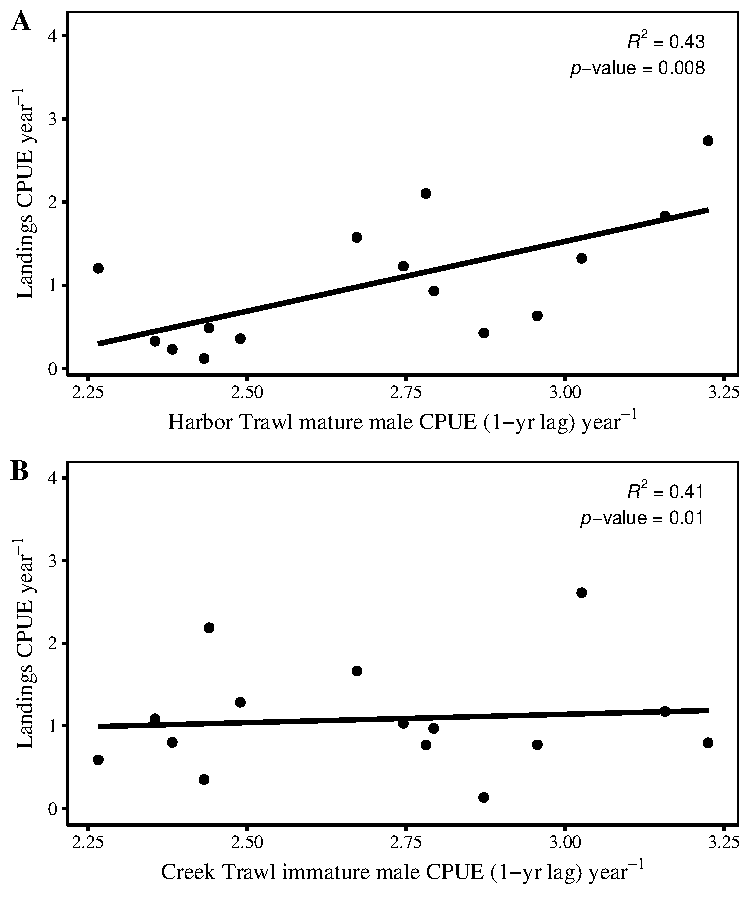
\includegraphics{NEWCh1_Figs_files/figure-latex/Figure 5-1.pdf}
\caption{Ordinary Least Squares regression plots of select significant
explanatory relatioships using lagged variables to Charleston Harbor
watershed Landings CPUEs. Mean annual effort corrected landings by (A)
Harbor Trawl mature males with a 1-yr lag, and (B) mean annual landings
CPUE by Creek Trawl immature males CPUE with a 1-yr. lag.}
\end{figure}

\end{document}
